\section{Module 2. Intensity inhomogeneity correction}
The aim of this module is to remove intensity inhomogeneity from MR image. Usually after MR imaging there are brighter and darker spots in the image of brain. The bias is very undesirable especially for the next modules such as segmentation and 3D imaging. The expected result of this module is that every kind tissue would be presented by approximately one shade of gray. As we never know how the bias map signal will look like, a method of removing it, which is be able to adapt to any shape of the inhomogeneity map is required. To achieve the goal, the following steps are taken. 
Firstly, the reconstructed image with intensity inhomogeneity is read (Fig. \ref{fig: Module2_1}).
\begin{figure}[H]
\centering{}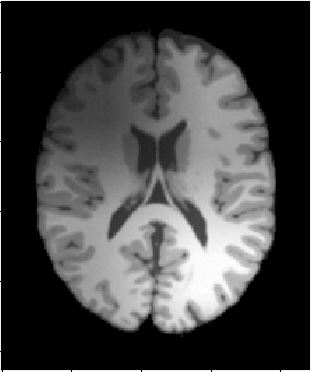
\includegraphics[scale=1]{figures/Module_02/m2_3}\caption{The original image with visible intensity inhomogeneity}. 
\label{fig: Module2_1}
\end{figure}
The next step is extracting the background of the image with Gaussian Filter of a size equal 2/3 the size of MRI image. In this step all the details corresponding to high frequency components are filtered out. The gaussian filter used in this part takes two variables. The first one is the size of the bandwidth and the second is the standard deviation sigma. For a picture of size 256x256 the size of the filter is set as 170x170 and the sigma is set as 20. Many tests have shown that too large sigma would reduce too much details from the background while too little sigma would leave too much details (Fig. \ref{fig: Module2_5}). The appropriate background extraction is shown in the Fig. \ref{fig: Module2_2}. 
\begin{figure}[H]
\centering{}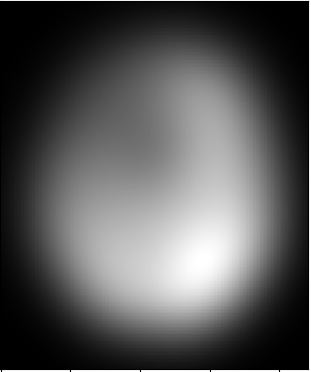
\includegraphics[scale=1]{figures/Module_02/m2_2}\caption{The filtered image with sigma = 5 (left) and sigma = 150(right)}. 
\label{fig: Module2_5}
\end{figure}
\begin{figure}[H]
\centering{}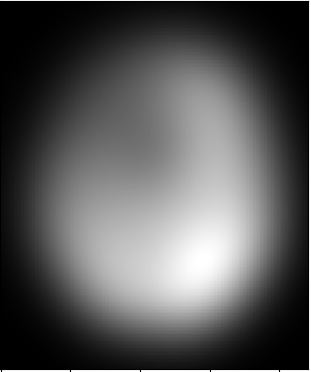
\includegraphics[scale=1]{figures/Module_02/m2_2}\caption{The image after Gaussian filtering}. 
\label{fig: Module2_2}
\end{figure}
Next there are 150 datapoints randomly selected from the background image. Every datapoint has 3 dimensions: x and y coordinates and z as a level of gray. They are used in next steps to fit a surface to the background. Following 3rd degree polynomial was set as the parametric equation of the surface:
\begin{equation}
\begin{aligned}
a+(b*x)+(c*y)+(d*x^{2})+(e*y^{2})+(f*x*y)+(g*x^{3})+(h*y^{3})+(i*x^{2}*y)+(i*x*y^{2})
\end{aligned}
\end{equation}
The fitting of the surface was performed with an $curve_fit$ function from the scipy module. $*describe in a few words how the function works*$ The equation is used to generate an image of bias field signal. The result is shown in the fig. \ref{fig: Module2_3}.
\begin{figure}[H]
\centering{}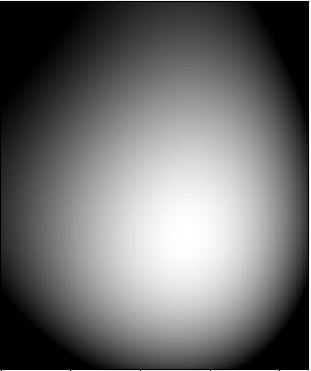
\includegraphics[scale=1]{figures/Module_02/m2_1}\caption{The surface fitted to the filtered image}. 
\label{fig: Module2_3}
\end{figure}
The last step is dividing each element of the original image by the corresponding element of the image of bias field performed with numpy function divide(). The result of this operation is shown in the fig. \ref{fig: Module2_4}.
\begin{figure}[H]
\centering{}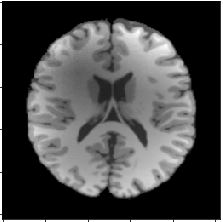
\includegraphics[scale=1]{figures/Module_02/m2_4}\caption{The result with intenstity bias removed}. 
\label{fig: Module2_4}
\end{figure}